% --- SLIDES : Introduction ---

\section{Introduction}

\begin{frame}
    \centering
    \Huge{\bfseries Introduction}
\end{frame}

\begin{frame}{Contexte du projet}

    % --- Premier bloc : Plateforme CryptoHack ---
    \begin{block}{La plateforme CryptoHack}
        \begin{itemize}
            \item Plateforme d'apprentissage dédiée à la \textbf{cryptographie moderne}.
            \item Résolution de défis à \textbf{difficulté croissante}.
        \end{itemize}
    \end{block}

    \vspace{0.5cm}

    % --- Deuxième bloc : Intérêt des CTF ---
    \begin{alertblock}{L'intérêt des challenges de type CTF (\textit{Capture The Flag})}
        \begin{itemize}
            \item \textbf{Principe :} \textit{Gamification} de l'apprentissage en cybersécurité.
            \item \textbf{Bénéfices :}
                \begin{itemize}
                    \item Ancrage des connaissances par la \textbf{pratique}.
                    \item Développement de \textbf{compétences techniques} (analyse, résolution de problèmes).
                \end{itemize}
        \end{itemize}
    \end{alertblock}

\end{frame}

\begin{frame}
    \frametitle{Organisation du projet}
    \framesubtitle{Planification}
    \centering
    % Remplacez 'path/to/image.png' par le chemin vers votre image.
    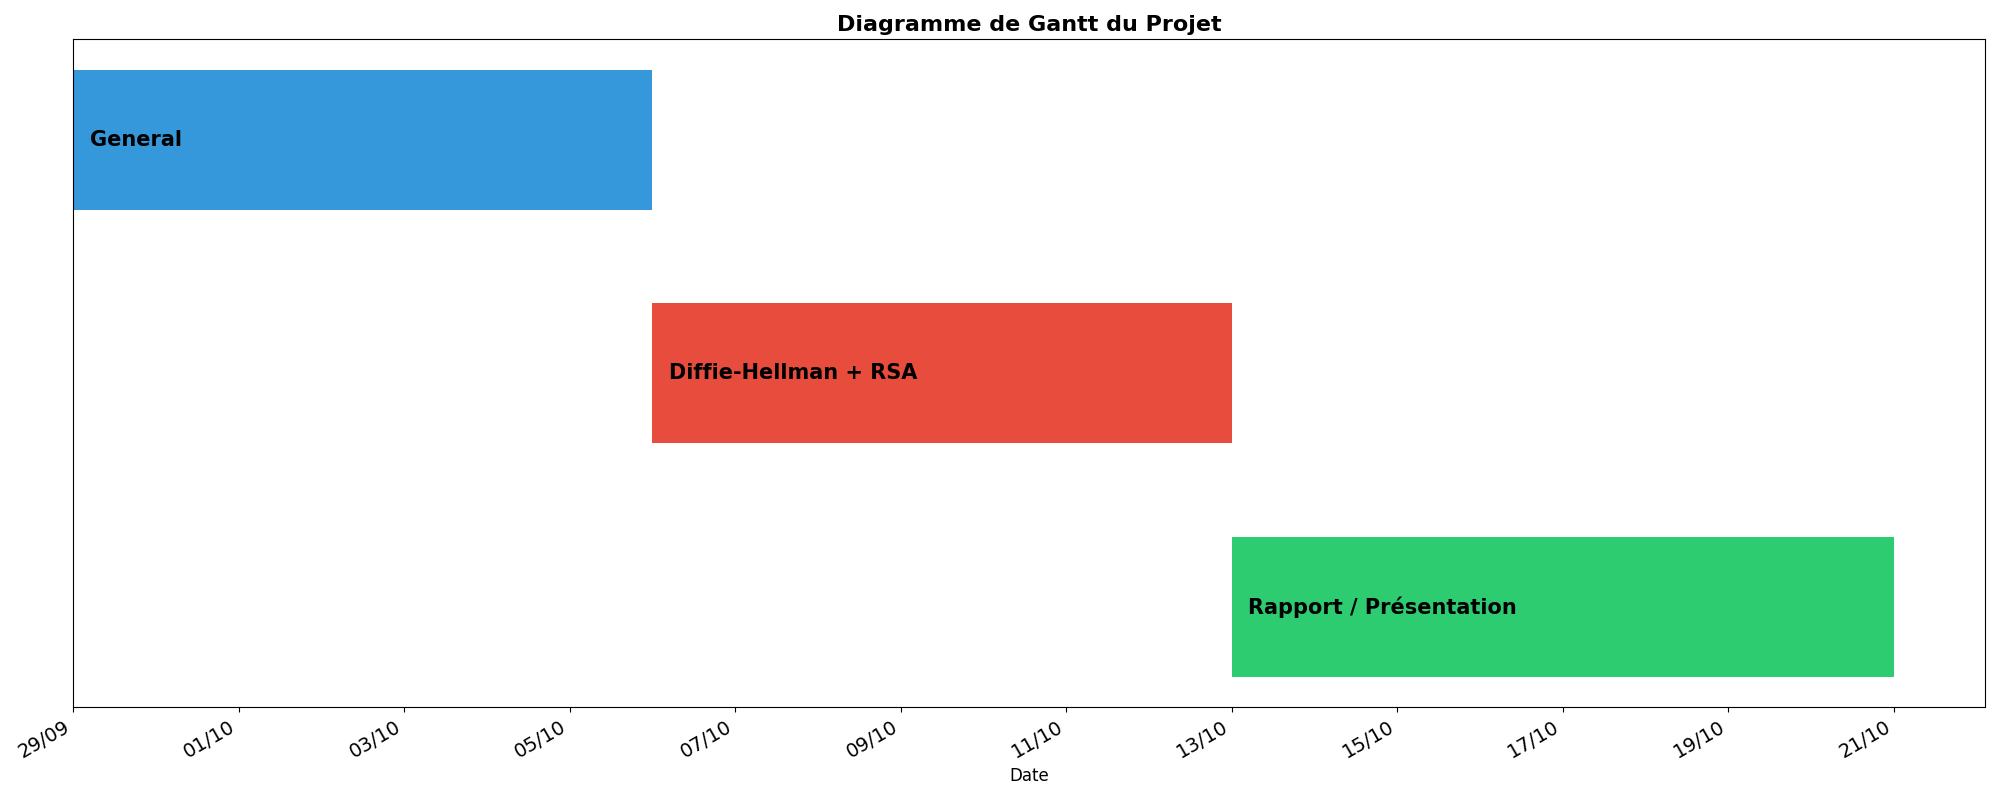
\includegraphics[width=\linewidth]{gantt.png}
\end{frame}

\begin{frame}
    \frametitle{Organisation du projet}
    \framesubtitle{Travailler en binôme}

    % --- Premier bloc : Répartition des tâches ---
    \begin{block}{Répartition des tâches individuelles}
        \centering
        \small
        \begin{tabular}{ll} 
            \textbf{} & \textit{Catégorie de challenges abordées} \\
            \textit{Victor} & General/\textbf{Encoding}, General/\textbf{XOR}, \textbf{Diffie-Hellman} \\
            \textit{Sébastien} & General/\textbf{Mathematics}, General/\textbf{Data Formats}, \textbf{RSA} \\
        \end{tabular}
    \end{block}

    \vspace{0.5cm} % Ajoute un peu d'espace entre les deux blocs

    % --- Deuxième bloc : Travail en commun ---
    \begin{alertblock}{Travail commun et collaboration}
        L'ensemble du projet a été géré via un dépôt Git partagé sur GitHub. Cette approche nous a permis de :
        \begin{itemize}
            \item \textbf{Centraliser le code} et les documents du projet.
            \item \textbf{Suivre les versions} pour éviter les conflits et les pertes de données.
            \item \textbf{Collaborer de manière asynchrone} sur les différentes parties du rapport et du code.
        \end{itemize}
    \end{alertblock}

\end{frame}